\documentclass[a4paper, 11pt]{article}
\usepackage{inputenc}
\usepackage{amsmath}
\usepackage{graphicx}
\usepackage[T1]{fontenc}
\usepackage{babel}
\RequirePackage[colorlinks, linkcolor=IBMblue, linktocpage=true, urlcolor=IBMblue, citecolor=IBMblue]{hyperref}
\hypersetup{pdfborder=1 1 1}
\usepackage{float} 
\usepackage{url}
\usepackage{caption}
\usepackage{multirow}
\usepackage{multicol}
\usepackage{listings}
\usepackage{subcaption}
\usepackage{empheq}
\usepackage{fancyhdr}
\usepackage{booktabs}
\usepackage{amssymb}
\usepackage{tikz, xifthen}
\usepackage{stmaryrd}

\usepackage{xcolor}
\definecolor{IBMblue}{HTML}{648fff}
\definecolor{IBMviolet}{HTML}{785ef0}
\definecolor{IBMpink}{HTML}{dc267f}
\definecolor{IBMorange}{HTML}{fe6100}
\definecolor{IBMyellow}{HTML}{ffb000}

\usepackage{setspace}
\usepackage{amsmath} % pour les notations mathématiques
\usepackage{algorithm} % pour l'environnement algorithm
\usepackage{algpseudocode} % pour l'environnement algpseudocode
\usepackage{enumitem}
\setlength{\hoffset}{-18pt}         
\setlength{\oddsidemargin}{0pt} % Marge gauche sur pages impaires
\setlength{\evensidemargin}{9pt} % Marge gauche sur pages paires
\setlength{\marginparwidth}{54pt} % Largeur de note dans la marge
\setlength{\textwidth}{481pt} % Largeur de la zone de texte (17cm)
\setlength{\voffset}{-18pt} % Bon pour DOS
\setlength{\marginparsep}{7pt} % Séparation de la marge
\setlength{\topmargin}{0pt} % Pas de marge en haut
\setlength{\headheight}{13pt} % Haut de page
\setlength{\headsep}{10pt} % Entre le haut de page et le texte
\setlength{\footskip}{27pt} % Bas de page + séparation
\setlength{\textheight}{708pt} % Hauteur de la zone de texte (25cm)
\setlength{\parindent}{10pt}
%Traits en haut et en bas des pages
\usepackage{fancyhdr}


\usepackage{unicode-math}

\ExplSyntaxOn
\bool_gset_true:N\g__um_upGreek_bool
\bool_gset_false:N\g__um_upgreek_bool
\bool_gset_true:N\g__um_bfupGreek_bool 
\bool_gset_false:N\g__um_bfupgreek_bool 
\bool_gset_false:N \g__um_bfliteral_bool
\bool_gset_true:N  \g__um_bfupLatin_bool
\bool_gset_true:N  \g__um_upLatin_bool
\bool_gset_false:N  \g__um_bfuplatin_bool
\bool_gset_false:N  \g__um_uplatin_bool
%more if needed ...
\ExplSyntaxOff

\usepackage[default, varnothing]{fontsetup}
\usepackage{fontspec-xetex}

\newcommand{\bm}{\symbf}
\newcommand{\di}{\ensuremath{\, \mathrm{d}}}
\newcommand{\e}{\ensuremath{\mathrm{e}}}

\pagestyle{fancy}
\fancyhead[L]{}
\fancyhead[R]{}
\renewcommand\footrulewidth{1pt}
\renewcommand\footrulewidth{1pt}
\fancyfoot[L]{\tiny Project Report}
\usepackage{lastpage}
\fancyfoot[R]{\tiny January 2024}
\fancyfoot[C]{\textbf{Page \thepage/\pageref{LastPage}}}
\lstnewenvironment{mathematicacode}[1][]
{
	\lstset{
		language=Mathematica,
		basicstyle=\small\ttfamily,
		numbers=left,
		numberstyle=\tiny,
		numbersep=5pt,
		frame=single,
		frameround=tttt,
		framexleftmargin=5pt,
		#1
	}
}
{}

\def\restriction#1#2{\mathchoice
	{\setbox1\hbox{${\displaystyle #1}_{\scriptstyle #2}$}
		\restrictionaux{#1}{#2}}
	{\setbox1\hbox{${\textstyle #1}_{\scriptstyle #2}$}
		\restrictionaux{#1}{#2}}
	{\setbox1\hbox{${\scriptstyle #1}_{\scriptscriptstyle #2}$}
		\restrictionaux{#1}{#2}}
	{\setbox1\hbox{${\scriptscriptstyle #1}_{\scriptscriptstyle #2}$}
		\restrictionaux{#1}{#2}}}
\def\restrictionaux#1#2{{#1\,\smash{\vrule height .8\ht1 depth .85\dp1}}_{\,#2}} 

\begin{document} 
	
	
	%----------------------------------------------------------------------------------------
	%	TITLE PAGE
	%----------------------------------------------------------------------------------------
	
	\begin{titlepage} % Suppresses displaying the page number on the title page and the subsequent page counts as page 1
		\newcommand{\HRule}{\rule{\linewidth}{0.5mm}} % Defines a new command for horizontal lines, change thickness here
		
		\centering % Centre everything on the page
		
		%------------------------------------------------
		%	Headings
		%------------------------------------------------
		
		\textsc{\LARGE \textbf{ENSEIRB-MATMECA}}\\[1cm] % Main heading such as the name of your university/college
		
		
		%\textsc{\large Minor Heading}\\[0.5cm] % Minor heading such as course title
		
		%------------------------------------------------
		%	Title
		%------------------------------------------------
		
		\vspace{5cm}
		
		\HRule\\[0.4cm]
		
		{\huge\bfseries\sffamily Solving the linear Boltzmann equation using Monte-Carlo methods \vspace{-0.4em}}\\[0.4cm] % Title of your document
		\HRule\\[1.5cm]
		
		{\huge\bfseries }
		
		\bigskip
		\bigskip
		
		\centering
		\Large{\textbf{Project lead by:}} \\
		\Large{C. Aumonier, A. Boucher, G. Doyen, K. El Maddah, G. Rodiere}
		
		%------------------------------------------------
		%	Date
		%------------------------------------------------
		{\vspace{3em}\Large  \textbf{Project supervised by:}}\\
		\Large{G. Poëtte}
		
		\vfill
		
		\begin{figure}[H]
			\begin{center}
				
\includegraphics[width=0.4\textwidth]{logo-embxinp.png}
			\end{center}
		\end{figure}
		
		\vspace{0,5cm}
		
		{\large January 2024} % Date, change the \today to a set date if you want to be precise
		
		%------------------------------------------------
		%	Logo
		%------------------------------------------------
		
		%\vfill\vfill
		%\includegraphics[width=0.2\textwidth]{placeholder.jpg}\\[1cm] % Include a department/university logo - this will require the graphicx package
		
		%----------------------------------------------------------------------------------------
		
		\vfill % Push the date up 1/4 of the remaining page
		
	\end{titlepage}
	
\tableofcontents

\newpage
	
\section{Introduction}



\subsection{Terms and definitions}

The transport equation plays a crucial role in describing the behavior of particles in various physical systems. One of its important derivatives, the linear Boltzmann equation, is governed by the evolution of particle distribution in phase space. In this project, a numerical solution for the linear Boltzmann equation is developed utilizing the Monte-Carlo method. The report is structured as follows:

\begin{itemize}
	\item \textbf{Transport Equation:} The fundamental transport equation is introduced, providing a basis for understanding the derivation of the linear Boltzmann equation.
	
	\item \textbf{Linear Boltzmann Equation:} Building upon the transport equation, the linear Boltzmann equation is explored, emphasizing its significance in characterizing particle transport phenomena.
	
	\item \textbf{Monte-Carlo Method for Linear Boltzmann Equation:} The approach to solving the linear Boltzmann equation using the Monte-Carlo method is presented, along with a discussion of the advantages and challenges associated with this numerical technique.
	
	\item \textbf{Semi-Analog Monte-Carlo Scheme:} A semi-analog Monte-Carlo scheme is introduced as an innovative strategy to enhance the efficiency and accuracy of simulations.
\end{itemize}

\subsection{Context and Applications}


The linear Boltzmann equation finds applications in a wide range of industrial and research contexts. Notable examples include its use in nuclear reactor physics, radiation shielding design, medical imaging, and astrophysics. Applications extend to industries such as nuclear energy, healthcare, and aerospace, where accurate simulations of particle transport are crucial for optimizing designs and ensuring safety protocols.

In the realm of academic research, the linear Boltzmann equation serves as a cornerstone in the study of rarefied gas dynamics, plasma physics, and neutron transport. Collaborations between universities, research institutions, and companies contribute to advancements in understanding and solving complex problems associated with particle transport phenomena.


\medbreak

This project aims to contribute to the broader understanding and application of the linear Boltzmann equation, with a focus on developing efficient numerical methods for solving this intricate problem.


\section{Mathematical analysis}

Here is a brief summary of the various existences and uniqueness of solutions based on different cases of equations to be solved. The primary source used is the Transport and Diffusion \cite{allaire:2019} document.

\subsection{Transport Equation}

In this section, the solutions of the transport equation, a particular case of the Boltzmann equation defined below, will be examined.
\begin{equation} \label{transport}
\frac{\partial f}{\partial t}(t,\bm{x})+\bm{v} \cdot \nabla_{\bm{x}} f(t,\bm{x}) + a(t,\bm{x})f(t,\bm{x}) = S(t,\bm{x}), \quad \bm{x} \in \bm{R}^N, \quad t>0.
\end{equation}
Where $f$ is solution of the equation, $a$ is a given damping or amplification rate, and $S$ is a given source term.

\subsubsection{Cauchy Problem}

Let the following Cauchy problem without absorption or source term be considered:
\[
\begin{cases}
\partial_t f(t,\bm{x})+\bm{v} \cdot \nabla_{\bm{x}} f(t,\bm{x})=0, \quad \bm{x} \in \bm{R}^N, \quad t>0.\\
f(0,\bm{x})) = f^{\mathrm{in}}(\bm{x})
\end{cases}
\]
where $f^{\mathrm{in}}(\bm{x})$ is the seeked initial value of $f$'s density. If $f^{\mathrm{in}} \in \mathcal{C}^1(\bm{R}^n)$, then using the characteristics method, the uniqueness of the solution $f \in \mathcal{C}^1(\bm{R}_+ \times \bm{R}^n)$ for the Cauchy problem can easily be demonstrated. This solution is given as follows:
\begin{equation}
f(t,\bm{x})=f^{\mathrm{in}}(\bm{x}-t\bm{v}) \quad \forall (t,\bm{x}) \in \bm{R}_+ \times \bm{R}^n 
\end{equation}
This time, a damping and a source term are considered, assuming they belong to $\mathcal{C}^1(\bm{R}_+ \times \bm{R}^n)$. The considered Cauchy problem is given as follows:
\[
\begin{cases}
\partial_t f(t,\bm{x})+\bm{v} \cdot \nabla_{\bm{x}} f(t,\bm{x}) + a(t,\bm{x})f(t,\bm{x}) = S(t,\bm{x}), \quad \bm{x} \in \bm{R}^N, \quad t>0.\\
f(0,\bm{x}) = f^{\mathrm{in}}(\bm{x})
\end{cases}
\]
Here the uniqueness of the solution remains unchanged so according to the same method, the solution is given by: 
\begin{equation}
f(t,\bm{x})= \left(f^{\mathrm{in}}(\bm{x}-t\bm{v}) + \int_0 ^t S(s,\bm{x}+(s-t)\bm{v})\di s \right) e^{-\int_0 ^t a(\tau,\bm{x}+(t-\tau)\bm{v})\di\tau} \quad \forall (t,\bm{x}) \in \bm{R}_+ \times \bm{R}^n
\end{equation}
Next, a partial demonstration of the previous formula is suggested, using the characteristics method. For more details, the reader is refered to \cite{allaire:2019}.

Let $\bm{y} \in \bm{R}^n$, and consider the characteristic curve emanating from $\bm{y}$ at $t=0$, given by:
\begin{equation}
\{(t,\gamma(t)),  t\geq 0\} , \text{ where } \gamma (t)=\bm{y}+t\bm{v}
\end{equation}
If $f \in \mathcal{C}^1(\bm{R}_+ \times \bm{R}^n)$ is the solution of the previous Cauchy problem, then $t \mapsto f(t,\gamma(t))$ is of $\mathcal{C}^1$ class on $\bm{R}_+$, and 
\[
\begin{aligned}
\frac{\di}{\di t}f(t,\gamma(t))&=\left(
\partial_t f + \bm{v} \cdot \nabla_{\bm{x}}  f\right)(t,\gamma(t))  \\ &= S(t,\gamma(t))-a(t,\gamma(t))f(t,\gamma(t)), \quad t>0.
\end{aligned}
\]
The previous partial differential equation is now reduced the following ordinary differential equation (ODE):
\[
\begin{cases}
u'(t)+\alpha(t)u(t)=\Sigma(t), \quad t>0,\\
u(0)=u^{\mathrm{in}}
\end{cases}
\]

The solution is calculated using the constant variation method:
\[ u(t) = u^{\mathrm{in}} e^{-A(t)} + \int_{0}^{t} e^{-(A(t)-A(s))}\Sigma(s)\di s, \text{ with } A(t)=\int_{0}^{t} \alpha (\tau) \di\tau. \]

The following expression is then obtained by applying the previously introduced method to the Cauchy problem along the characteristic curve from $\bm{y}$ at $t=0$:

\begin{equation}
f(t,\bm{y}+t\bm{v}) = f^{\mathrm{in}}(\bm{y}) e^{\int_{0}^{t}a(\tau,\bm{y}+\tau \bm{v})\di\tau} + \int_{0}^{t} e^{\int_{0}^{t}a(\tau,\bm{y}+\tau \bm{v})d\tau}S(s,\bm{y}+s\bm{y})\di s, \quad \bm{y}\in \bm{R}^n, t \geq 0.
\end{equation}

Finally, the expected expression is deduced by replacing the dummy variable $\bm{y}$ with $\bm{y}-t\bm{v}$.

\subsubsection{Boundary Value Problems}

In the previous section, outcomes relevant to the exploration of unrestricted spatial variables in $\bm{R}^n$ were provided. However, for the majority of physical problems, this spatial unrestriction has no sens. That is why a problem of the boundary value type is more interesting. In this section, the set $\Omega$, which is an open set with a $\mathcal{C}^1$ boundary in $\bm{R}^n$ is considered. Additionally, $\bm{v} \in \bm{R}^n\backslash \{0\}$ is considered.

\paragraph{Special Case without Absorption or Source Term}

Let $\Omega$ be convex, $f_b^- \in \mathcal{C}^1(\bm{R}_+ \times \partial \Omega^-)$ and $f^{\mathrm{in}} \in \mathcal{C}^1(\overline{\Omega})$, where $\partial \Omega^- = \{\bm{x}\in\partial \Omega~ | ~ \bm{v}\cdot \bm{n}_x<0\}$, then the problem:
\[
\begin{cases}
\partial_t f(t,\bm{x})+\bm{v} \cdot \nabla_{\bm{x}} f(t,\bm{x})=0, \quad \bm{x} \in \bm{R}^N, \quad t>0.\\
\restriction{f}{\partial \Omega}= f_b^-\\
\restriction{f}{t=0}= f^{\mathrm{in}}
\end{cases}
\]
has a unique solution $f \in \mathcal{C}^1(\bm{R}_+ \times \Omega)$ and $f \in \mathcal{C}^0(\bm{R}_+ \times \overline{\Omega})$ if and only if $\forall \bm{y} \in \partial \Omega^-,$
\[ f_b^-(0,\bm{y}) = f^{\mathrm{in}}(\bm{y}), \quad \partial_t f_b^-(t,\bm{y})+\bm{v} \cdot \nabla f^{\mathrm{in}}(\bm{y})=0. \]

The expression of the solution is then given by: 
\[
f(t,\bm{x})= 
\begin{cases}
f^{\mathrm{in}}(\bm{x}-t\bm{v}) \quad &\mathrm{if}~ t \leq \tau_{\bm{x}} ,\\
f_b^-(t-\tau_{\bm{x}},\bm{x}-\tau_{\bm{x}}\bm{v}) \quad &\mathrm{if}~ t > \tau_{\bm{x}} ,
\end{cases}
\]
with $\tau_{\bm{x}}= \inf \{t \geq 0~ | ~ \bm{x}-t\bm{v} \notin \overline{\Omega}\}$

\paragraph{With Absorption and Source Term}

Let still $\Omega$ be convex, with $f_b^- \in \mathcal{C}^1(\bm{R}_+ \times \partial \Omega^-)$, $f^{\mathrm{in}} \in \mathcal{C}^1(\overline{\Omega})$, $a$, and $S$ $\in \mathcal{C}^1(\bm{R}_+ \times \overline{\Omega})$. 
\medbreak

For all $\bm{y} \in \partial \Omega^-$:
\[
\begin{aligned}
f_b^-(0,\bm{y}) &= f^{\mathrm{in}}(\bm{y}), \\
S(0,\bm{y}) &= \partial_t f_b^-(0,\bm{y}) + \bm{y} \cdot \nabla_{\bm{x}} f^{\mathrm{in}}(\bm{y}) + a(0,\bm{y})f^{\mathrm{in}}(\bm{y})
\end{aligned}
\]

In this case, the problem becomes:
\[
\begin{cases}
\partial_t f(t,\bm{x})+\bm{v} \cdot \nabla_{\bm{x}} f(t,\bm{x})+ a(t,\bm{x})f(t,\bm{x})=S(t,\bm{x}), \quad \bm{x} \in \bm{R}^N, \quad t>0.\\
\restriction{f}{\partial \Omega}= f_b^-\\
\restriction{f}{t=0}= f^{\mathrm{in}}
\end{cases}
\]
and has a unique solution $f \in \mathcal{C}^1(\bm{R}_+ \times \Omega)$ and $f \in \mathcal{C}^0(\bm{R}_+ \times \overline{\Omega})$. The expression for $f$ is then:
\[
\boxed{
	\begin{aligned}
	f(t,\bm{x}) &= \mathbf{1}_{t \leq \tau_{\bm{x}}} f^{\mathrm{in}} (\bm{x}-t\bm{v}) \exp\left(-\int_0^t a(s,\bm{x}+(s-t)\bm{v})\di s\right) \\
	&\quad + \mathbf{1}_{t > \tau_{\bm{x}}} f_b^- (t-\tau_{\bm{x}},\bm{x}-\tau_{\bm{x}} \bm{v}) \exp\left(-\int_{t-\tau_{\bm{x}}}^t a(s,\bm{x}+(s-t)\bm{x})\di s\right) \\
	&\quad + \int_{\min(0,t-\tau_{\bm{x}})}^t \exp\left(-\int_{s}^{t}a(\tau,\bm{x}+(\tau-t)\bm{v})\di\tau\right) S(s,\bm{x}+(s-t)\bm{v})\di s
	\end{aligned}}
\]

\subsubsection{Generalized Solutions}

In this section, $\Omega$ is not necessarily convex. This implies that the continuity of potential solutions is not guaranteed. However, in practice, these cases must be addressed. Below, the concept of generalized solutions is defined, which allows to handle this issue without resorting to the theory of distributions.

\paragraph{Definition}

Let $\Omega$ be an open set with a $\mathcal{C}^1$ boundary in $\bm{R}^n$, and let $a$ and $S$ be continuous on $\bm{R}_+ \times \Omega$. $f$ is a generalized solution of the problem $(1)$ if and only if the function $s \mapsto f(t+s,\bm{x}+s\bm{v})$ is of class $\mathcal{C}^1$ almost everywhere in $(t,\bm{x}) \in \bm{R}_+ \times \Omega$ and satisfies:

\begin{equation}
\left(\frac{\di}{\di s} +a(t+s,\bm{x}+s\bm{v})\right)f(t+s,\bm{x}+s\bm{v}) = S(t+s,\bm{x}+s\bm{v}) \quad (t+s,\bm{x}+s\bm{v}) \in \bm{R}_+^* \times \Omega.
\end{equation}


Now let $\Omega$ be an open set with a $\mathcal{C}^1$ boundary in $\bm{R}^n$, and let $a$ and $S$ be continuous on $\bm{R}_+ \times \Omega$. Let $f_b^- \in \mathbf{L}_{loc}^{\infty}(\bm{R}_+ \times \partial \Omega^-)$ and $f^{\mathrm{in}} \in \mathbf{L}_{loc}^{\infty}(\overline{\Omega})$.
In this case, the problem:
\[
\begin{cases}
\partial_t f(t,\bm{x})+\bm{v} \cdot \nabla_{\bm{x}} f(t,\bm{x})+ a(t,\bm{x})f(t,\bm{x})=S(t,\bm{x}), \quad \bm{x} \in \bm{R}^N, \quad t>0.\\
\restriction{f}{\partial \Omega}= f_b^-\\
\restriction{f}{t=0}= f^{\mathrm{in}}
\end{cases}
\]
has a unique generalized solution. The formula for this solution is the same as in the previous case, i.e., almost everywhere in $(t,\bm{x}) \in \bm{R}_+ \times \Omega$:
\[
\boxed{
	\begin{aligned}
	f(t,x) &= \mathbf{1}_{t \leq \tau_{\bm{x}}} f^{\mathrm{in}} (\bm{x}-t\bm{v}) \exp\left(-\int_0^t a(s,\bm{x}+(s-t)\bm{v})\di s\right) \\
	&\quad + \mathbf{1}_{t > \tau_{\bm{x}}} f_b^- (t-\tau_{\bm{x}},\bm{x}-\tau_{\bm{x}} \bm{v}) \exp\left(-\int_{t-\tau_{\bm{x}}}^t a(s,\bm{x}+(s-t)\bm{v})\di s\right) \\
	&\quad + \int_{\min(0,t-\tau_{\bm{x}})}^t \exp\left(-\int_{s}^{t}a(\tau,\bm{x}+(\tau-t)\bm{v})\di\tau\right) S(s,\bm{x}+(s-t)\bm{v})\di s
	\end{aligned}}
\]


\subsection{Linear Boltzmann Equation}

In this section, a particular attention is paid on the actual Boltzmann equation. This integro-differential equation is described hereafter.

\begin{equation} \label{Boltzmann}
\partial_t f(t,\bm{x},\bm{v})+ \bm{v} \cdot \nabla_{\bm{x}} f(t,\bm{x},\bm{v}) + a(t,\bm{x})f(t,\bm{x},\bm{v}) = \int_{\bm{R}^n} k(t,\bm{x},\bm{v},\bm{w})f(t,\bm{x},\bm{w})\di\mu(\bm{w})+Q(t,\bm{x},\bm{v}).
\end{equation}

To simplify notations, this equation will be written as: 
\[ \partial_t f + \bm{v} \cdot \nabla_{\bm{x}} f + a f = \mathcal{K} f +Q  \]

Here, $\bm{v}$ and $k$ are given continuous functions. The range of possibilities for the velocity $\bm{v}$ is very diverse due to the variety of physical problems that can be considered. Therefore, the notation $d\mu(\bm{w})$ encompasses all these possibilities by incorporating a weight function. The major difference from the transport equation is that, this time, exchange phenomena are considered, and thus, $\bm{v}$ can not be seen as a simple parameter.

In this section, the exact expression of the solutions can not be highlighted because the characteristics method yields another integral equation involving the solution.


\paragraph{Definition}

Let $Q$ be continuous on $(0,T)\times \Omega \times \bm{R}^n$. $f$ is a generalized solution of the problem \eqref{Boltzmann} if and only if, $\forall (t,\bm{x},\bm{v}) \in (0,T)\times \Omega \times \bm{R}^n$, the function $ s \mapsto f(t+s,\bm{x}+s\bm{v},\bm{v}) $	is of class $\mathcal{C}^1$ for all $\bm{x}+s\bm{v} \in \Omega$ and satisfies:
\[ \left(\frac{\di}{\di s} +a(t+s,\bm{x}+s\bm{v},\bm{v})\right)f(t+s,\bm{x}+s\bm{v},\bm{v}) = (\mathcal{K}f+ Q)(t+s,\bm{x}+s\bm{v},\bm{v}). 
\]
For all $s \in \bm{R}$ such that $\bm{x} +s\bm{v} \in \Omega$.

\subsubsection{Cauchy Problem}

Let $f^{\mathrm{in}} \in \mathbf{C}_b(\bm{R}^n \times \bm{R}^n)$ and $Q \in \mathbf{C}_b((0,T) \times \bm{R}^n \times \bm{R}^n)$. Also, let $0 \leq a \in \mathbf{C}_b((0,T) \times \bm{R}_x^n \times \bm{R}_v^n)$ and $0 \leq k \in \mathbf{C}_b((0,T) \times \bm{R}_x^n \times \bm{R}_v^n \times \bm{R}_w^n)$. The notation $\mathbf{C}_b(X)$ denotes the set of bounded continuous functions on $X$ with values in $\bm{R}$.
\medbreak
Now assuming that:  
\[ \underset{(t,x,v) \in ]0,T[ \times \bm{R}^n \times \bm{R}^n}{\sup} \int_{\bm{R}^n} k(t,\bm{x},\bm{v},\bm{w}) \, \di\mu(\bm{w}) < +\infty, \]
the problem:
\[
\begin{cases}
\partial_t f +\bm{v} \cdot \nabla_{\bm{x}} f + a f = \mathcal{K} f + Q \quad (t,\bm{x},\bm{v}) \in (0,T) \times \bm{R}^n \times \bm{R}^n\\
\restriction{f}{t=0}= f^{\mathrm{in}}
\end{cases}
\]
has a unique generalized solution $f \in \mathbf{C}_b((0,T) \times \bm{R}^n \times \bm{R}^n)$.

\subsubsection{Boundary Value Problem}

The set $\Gamma_-$ is defined as $\Gamma_-= \{(\bm{x},\bm{v}) \in \partial \Omega \times \bm{R}^n ~ | ~ \bm{v}\cdot \bm{n}_{\bm{x}}<0\}$. Let:
\begin{itemize}
	\item $f^{\mathrm{in}} \in \mathbf{C}_b(\overline{\Omega} \times \bm{R}^n)$, $f_b^- \in \mathbf{C}_b([0,T] \times \Gamma_-)$ such that $f_b^-(0,\bm{y},\bm{v})=f^{\mathrm{in}}(\bm{y},\bm{v}) \quad \forall (\bm{y},\bm{v}) \in \Gamma_-$
	\item $Q \in \mathbf{C}_b([0,T] \times \overline{\Omega} \times \bm{R}^n)$
	\item $0 \leq a \in \mathbf{C}_b(\bm{R}_+ \times \Omega_x \times \bm{R}_v^n)$ and $0 \leq k \in \mathbf{C}_b(\bm{R}_+ \times \Omega_x^n \times \bm{R}_v^n \times \bm{R}_w^n)$
\end{itemize}

Then the problem
\[
\begin{cases}
\partial_t f+\bm{v} \cdot \nabla_{\bm{x}} f +af =   \mathcal{K} f +Q \quad (t,\bm{x},\bm{v}) \in (0,T) \times \Omega \times \bm{R}^n\\
\restriction{f}{t=0}= f^{\mathrm{in}}\\
\restriction{f}{\Gamma^-}=f_b^-
\end{cases}
\]
has a unique generalized solution $f \in \mathbf{C}_b([0,T] \times \Omega \times \bm{R}^n)$.

\section{The use of Monte-Carlo methods to solve the linear Boltzmann equation}


To facilitate the introduction of a numerical scheme, the equation is modified into an integral form. The different steps are detailed in this section.

The transport equation in an infinite medium with its corresponding deterministic collisional component\cite{lapeyre_methodes_1998} can be expressed as:
\begin{equation}
\partial _t u(x,t,\bm{v}) + \bm{v} \cdot \nabla u(x,t,\bm{v}) + v\sigma_t (x,t,\bm{v})u(x,t,\bm{v})= v\sigma_s(x,t,\bm{v})\int P (x,t,\bm{v},\bm{v}')u(x,t,\bm{v}')\di\bm{v}' \label{ref11}
\end{equation}

Where 
\begin{equation*}
\sigma_s (\bm{x},t,\bm{v})= \int \sigma_s (\bm{x},t,\bm{v},\bm{v}')d\bm{v}', \quad  P (\bm{x},t,\bm{v},\bm{v}')= \frac{\sigma_s (\bm{x},t,\bm{v},\bm{v}')}{\sigma_s (\bm{x},t,\bm{v})}
\end{equation*}

This approach involves a series of variable changes. The initial step involves re-expressing the transport equation \ref{ref11} with respect to a characteristic $x + vt$. As a result, it transforms into:
\begin{equation}
\partial _s u(\bm{x}+\bm{v}s,s,\bm{v}) = -v\sigma_t (\bm{x}+\bm{v}s,s,\bm{v})u(x+\bm{v}s,s,\bm{v}) + v\sigma_s(\bm{x}+\bm{v}s,s,\bm{v})\int P (\bm{x}+\bm{v}s,s,\bm{v},\bm{v}')u(\bm{x}+\bm{v}s,s,\bm{v}')\di\bm{v}'
\end{equation}
By multiplying both sides of the equation by $e^{\int _0^s v\sigma_t (\bm{x} + \bm{v}\alpha,\alpha, v) \di\alpha}$, the equation becomes:
\begin{equation}
\partial _s \left[u(\bm{x}+\bm{v}s,s,\bm{v})e^{\int _0^s v\sigma_t (\bm{x} + \bm{v}\alpha,\alpha, v) \di\alpha}\right] = e^{\int _0^s v\sigma_t (\bm{x} + \bm{v}\alpha,\alpha, v) \di\alpha} v\sigma_s(\bm{x}+\bm{v}s,s,\bm{v})\int P (\bm{x}+\bm{v}s,s,\bm{v},\bm{v}')u(\bm{x}+\bm{v}s,s,\bm{v}')\di\bm{v}' \label{ref12}
\end{equation}
After integrating on $[0, t]$, the equation now yields:
\begin{multline}
u(\bm{x}+\bm{v}t,t,\bm{v}) = u_0(x, \bm{v}) \exp\left(- \int_{0}^{t} v\sigma_t\left(\bm{x} + \bm{v} \alpha, \alpha, \bm{v}\right) \di\alpha\right) \\
+ \int_{0}^{t} \int v\sigma_s\left(\bm{x} + \bm{v}s, s, \bm{v}\right) u\left(\bm{x} + \bm{v}s, s, \bm{v}'\right) e^{- \int_s^t v\sigma_t\left(\bm{x} + \bm{v} \alpha, \bm{v}\right) \di\alpha} P\left(\bm{x} + \bm{v} s, s, \bm{v}, \bm{v}'\right) \di\bm{v}'\di s 
\end{multline}
And then:
\begin{multline}
u(x,t,\bm{v}) = u_0(\bm{x} - \bm{v}t, \bm{v}) \exp\left(- \int_{0}^{t} v\sigma_t\left(\bm{x} - \bm{v}(t - \alpha), \alpha, \bm{v}\right) \di\alpha\right) \\
+ \int_{0}^{t} \int v\sigma_s\left(\bm{x} - \bm{v}(t - s), s, \bm{v}\right) u\left(\bm{x} - \bm{v}(t - s), s, \bm{v}'\right) e^{- \int_s^t v\sigma_t\left(\bm{x} - \bm{v}(t - \alpha), \bm{v}\right) \di\alpha} P\left(\bm{x} - \bm{v}(t - s), s, \bm{v}, \bm{v}'\right) \di\bm{v}'\di s \label{ref1}
\end{multline}
But also:
\begin{multline}
\exp\left(- \int_{0}^{t} v\sigma_t\left(\bm{x} - \bm{v}(t - \alpha), \alpha, \bm{v}\right) \di\alpha\right) = \exp\left(- \int_{0}^{t} v\sigma_t\left(\bm{x} - \bm{v} \alpha,t- \alpha, \bm{v}\right) \di\alpha\right) \\ = \int _t^\infty  v\sigma_t\left(\bm{x} - \bm{v} s,t- s, \bm{v}\right)
\exp\left(- \int_{0}^{s} v\sigma_t\left(\bm{x} - \bm{v} \alpha,t- \alpha, \bm{v}\right) \di\alpha\right) \di s
\end{multline}
Then the integral representation of \ref{ref11} is provided by:

\begin{multline}
u(\bm{x},t,\bm{v}) =  \int _t^\infty  u_0(\bm{x} - \bm{v}t, \bm{v}) v\sigma_t\left(\bm{x} - \bm{v} s,t- s, \bm{v}\right) \exp\left(- \int_{0}^{s} v\sigma_t\left(\bm{x} - \bm{v} \alpha,t- \alpha, \bm{v}\right) \di\alpha\right) \di s\\
+ \int_{0}^{t} \int v\sigma_s\left(\bm{x} - \bm{v}(t - s), s, \bm{v}\right) u\left(\bm{x} - \bm{v}(t - s), s, \bm{v}'\right) e^{- \int_s^t v\sigma_t\left(\bm{x} - \bm{v}(t - \alpha), \bm{v}\right) \di\alpha} P\left(\bm{x} - \bm{v}(t - s), s, \bm{v}, \bm{v}'\right) \di\bm{v}'\di s \label{ref13}
\end{multline}


\section{Semi analog Monte-Carlo scheme}

Developing a Monte-Carlo scheme involves introducing a group of random variables along with their associated probability measure to express \eqref{ref13} as an expectation. The selection of this set of random variables is not unique, resulting in various Monte-Carlo schemes with distinct properties. In this project we used one of them, the so-called Semi-analog scheme. The algorithm 1 describe this method.



This method is described as backward. In fact, we first initialize $S_p$, the remaining lifetime of the particle, to $t$, and it will decrease to zero. Here, we adopt a general form for the boundary conditions. In the program we developed, we have tried various conditions: Periodic boundary conditions (which are not truly significant in a physical problem but can be interpreted as an infinite environment), and Elastic boundary conditions.

At line 11, we sample $\tau$ using the function: $\tau = \frac{-\ln(\mathcal{U}(0,1))}{\sigma_t \sqrt{v^2}}$. If $\tau$ is greater than $s_p$, then the particle is moved, its lifetime is set to zero, and its contribution is updated. Otherwise, the particle is moved, its speed is sampled on the unit sphere, its lifetime is updated, and finnaly its weight is changed.

\begin{algorithm}
	\caption{Semi-analog backward Monte-Carlo scheme algorithm}
	\begin{algorithmic}[1]
		\State Let $u(\bm{x}, t, \bm{v}) \gets 0$;
		\For{$p \in \llbracket 1 ; N_{Monte-Carlo} \rrbracket$}
		\State set $s_p = t$
		\State set $\bm{x}_p = \bm{x}$
		\State set $\bm{v}_p = \bm{v}$
		\State set $w_p(t) = N_{Monte-Carlo}$
		\While{$s_p > 0$ and $w_p > 0$}
		\If{$\bm{x}_p \not \in \mathcal{D}$}
		\State apply\_BCs$(\bm{x}_p, s_p, \bm{v}_p)$
		\EndIf
		\State Sample $\tau \leadsto f_\tau(\bm{x}_p, s_p, \bm{v}_p, s) \di s$
		
		\If{$\tau < s_p$}
		\Comment{{\scriptsize Scattering/Collision}}
		\State $w_p \gets \frac{\sigma_s(\bm{x}_p, s_p - \tau, \bm{v}_p)}{\sigma_t(\bm{x}_p, s_p - \tau, \bm{v}_p)} w_p$
		\State Sample $\bm{v}_p \leadsto P_{\bm{V}'}^s(\bm{x}_p, s_p, \tau, \bm{v}_p, \bm{v}') \di \bm{v}'$
		\State $\bm{x}_p \gets \bm{x}_p + \bm{v}_p \tau$
		\State $s_p \gets s_p - \tau > 0$
		
		\Else
		\Comment{{\scriptsize Census/Contribution}}
		\State $\bm{x}_p \gets \bm{x}_p + s_p \bm{v}_p$
		\State $s_p \gets 0$
		\State $u(\bm{x}, t, \bm{v}) += w_p u_0(\bm{x}_p, \bm{v}_p)$
		\EndIf
		\EndWhile
		\EndFor
	\end{algorithmic}
\end{algorithm}






\section{Code architecture}


\begin{figure}[H]
	\centering
	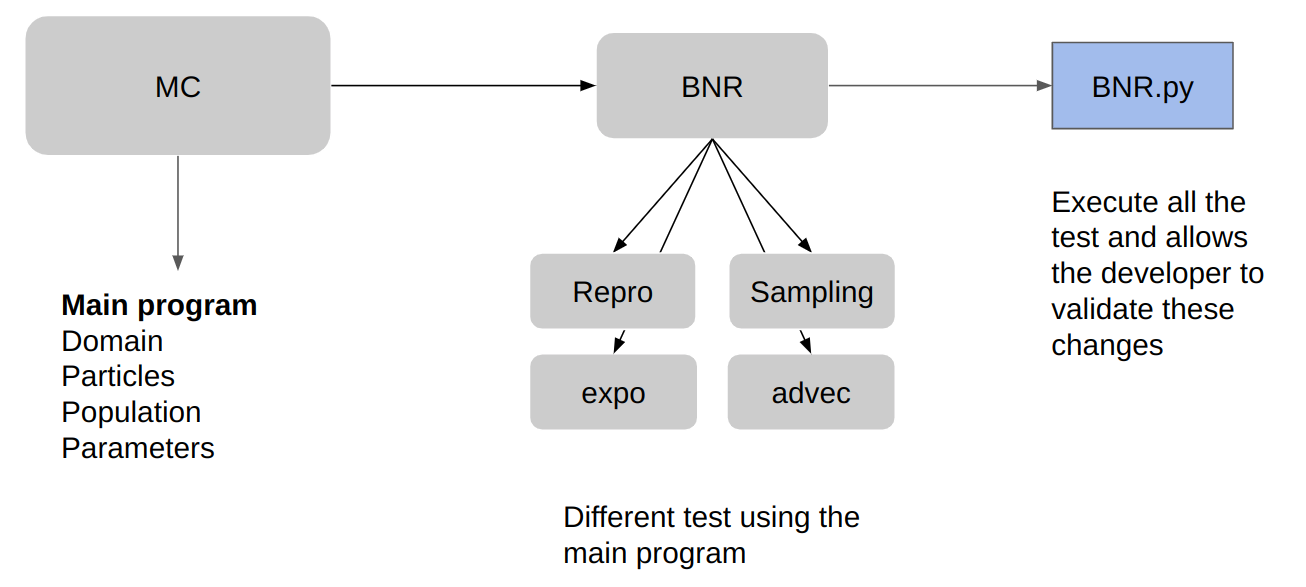
\includegraphics[width=1.0\linewidth]{codestruct.png}
	\caption {Code architecture}
	\label{fig:code}
\end{figure}

The figure \ref{fig:code} represent the structure of our implementation. The \textbf{Main program} is used for several computation, \textbf{Domain} set up the boundary condition, initial condition and the sampling of $\bm{v}_p$ and $\tau$. \textbf{Particles} set up the semi analog scheme, \textbf{Population} Move all the particles and \textbf{Parameters} initializes the parameters.

\paragraph{Regression suite}

In order to facilitate the implementation and the improvement of the code, a regression suite has been established. The script \textbf{BNR.py} execute all the test sequentially and relative messages to each test are print in the console. The user can then decide if the test are passed or not.

The reproducibility test compute 2 times the solution for one $t$ fixed and checks if the both results are similar or not.

The sampling test a high number of speed $\bm{v}_p$ checking if this speed is really on the unit sphere by using the Kolmogorov-Smirnov law.

The advection test used a computation of the main program with $\sigma_t=\sigma_s=0$. We are in the case of the advection described previously and we compare the result computed with the known exact-solution.

The exponential test used a computation of the main program with constants $\sigma_t \neq 0$ and $\sigma_s \neq 0$. With this configuration we can calculate the integral of the exact solution as:
\[ \int_{\Omega} \bar{U}(t, \bm{x})\di \bm{x}=\int_{\Omega} \bar{U}_0(\bm{x}) \di \bm{x} ~ \e^{-v(\sigma_t-\sigma_s)t} \]
where $\bar{U} = \int U(\omega) \di \omega$, and compare to the computed solution.


\section{Conclusion}

First and foremost, we would like to express our sincere appreciation to our supervisor, Gael Poette, whose exceptional support was evident through his constant presence and responsiveness throughout our research.

This project provided a unique opportunity to work on Monte-Carlo methods. Accustomed to working with partial differential equations, the adoption of this new method for solving equations presented a stimulating challenge over the course of these four months. Collaborating in a group of five within such a limited timeframe posed its own set of challenges, but we successfully brought the project to completion.

The work we accomplished enabled us to gain a deeper understanding of high-dimensional equation solving, a skill set that will undoubtedly prove invaluable in our future professional lifes.
	
	
	
\newpage

\nocite{*}
\bibliography{biblio}
\bibliographystyle{unsrt}
	
\end{document}